\clearpage\onecolumn
\section{Worked Dismantling and Repair}
All examples below use configuration \texttt{exp-d1-arm-2}. Its six modules
form the chain foundation, mount, shoulder, elbow, wrist, tool. Task IDs
are formed by prefixing the family with \texttt{h3-exp-d1-arm-2-}.
The images come from the original application's canvas; no interface
labels are included. Every intermediate fact set and image hash is
archived in \texttt{publication-capture.json}.

\begin{center}
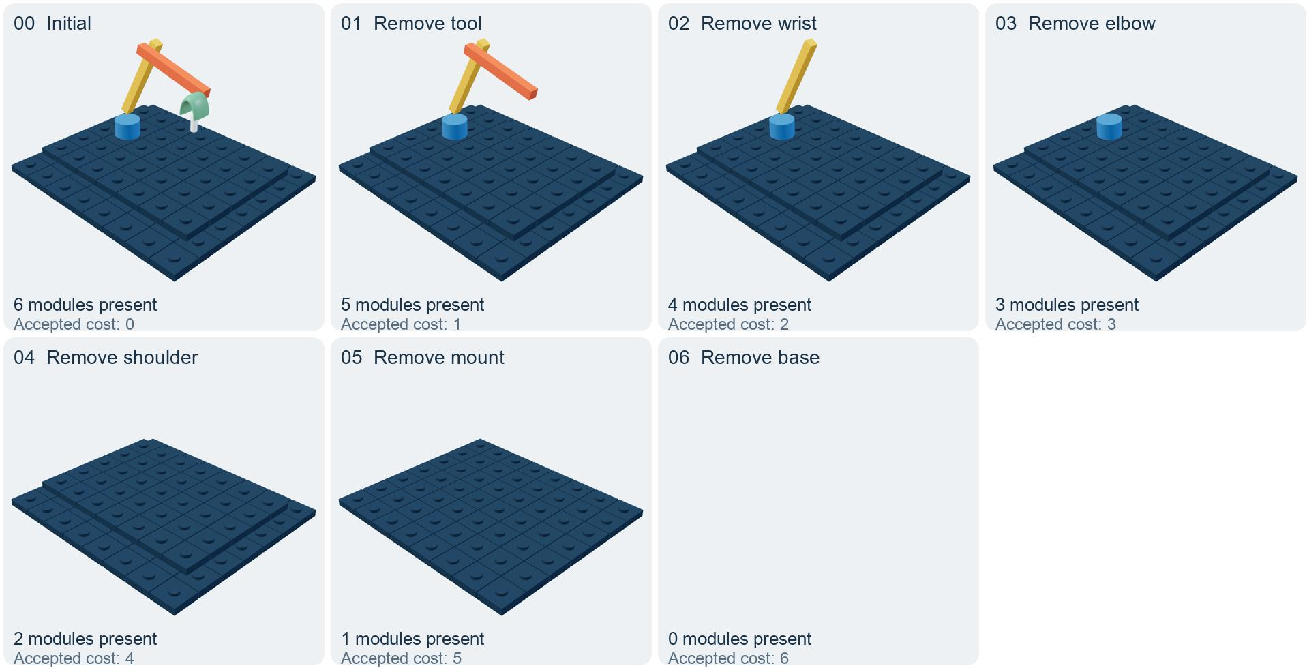
\includegraphics[width=\textwidth]{figures/publication-disassembly.pdf}
\end{center}
\noindent\textbf{Dismantling.}
Each action requires its target to be present and its direct children
to be absent. All six removals cost one unit each. The target's presence
fact is deleted and its \texttt{removed} marker is added. The visible module
is removed by the replay renderer. The reference order below is forced
by this serial dependency chain; branched models can admit alternative
legal orders.

\begin{center}\small
\begin{tabularx}{\textwidth}{rllX}
\toprule Step & Action target & Required absent child & Related task interpretation\\\midrule
1 & Tool & None (leaf) & \texttt{remove}: choose a leaf; \texttt{parent}: identify the wrist.\\
2 & Wrist & Tool & \texttt{degree}/\texttt{boundary}: identify incident structural interfaces.\\
3 & Elbow & Wrist & Apply the same dependency rule to the reduced assembly.\\
4 & Shoulder & Elbow & \texttt{counterfactual}: separately assess anchored reachability.\\
5 & Mount & Shoulder & Verify that no dependent module remains attached.\\
6 & Foundation & Mount & Reach the disassembly goal: every module absent.\\
\bottomrule
\end{tabularx}
\end{center}
The task families in the final column provide a conceptual mapping.
They are separate fixed questions on the original configuration,
not newly generated questions at every intermediate frame.
The \texttt{prefix} family tests the first predecessor violation in
an assembly sequence; full disassembly instead executes all proposed
removals through the interpreter.

\begin{center}
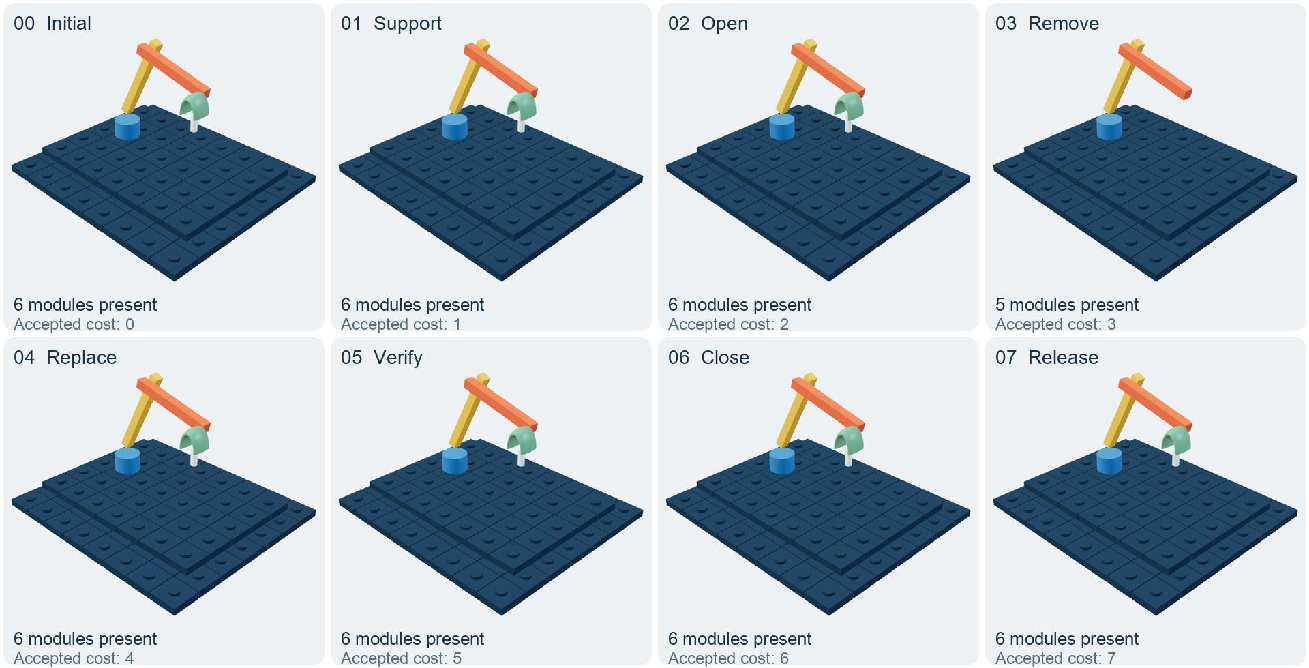
\includegraphics[width=\textwidth]{figures/publication-repair.pdf}
\end{center}
\noindent\textbf{Service repair.}
Let $u$ denote \texttt{cell-0-tool}. Initially \texttt{fault:$u$}
and \texttt{closed:$u$} are present. Every action below has unit
cost and forbids its own completion marker. A completion marker is
written as \texttt{done:action:$u$}. The budget is seven and the goal
is \texttt{repaired:$u$}.

\begin{center}\small
\begin{tabularx}{\textwidth}{rllXX}
\toprule Step & Action & Required fact & Effect beyond its completion marker & Task interpretation\\\midrule
1 & support & fault:$u$ & No geometric effect & Establish the service support prerequisite.\\
2 & open & done:support:$u$ & No geometric effect & Establish access in the symbolic contract.\\
3 & remove & done:open:$u$ & Hide the tool module & Execute the removal after access.\\
4 & replace & done:remove:$u$ & Show the tool module & Restore the module before checking it.\\
5 & verify & done:replace:$u$ & Delete fault:$u$ & Clear the fault only after replacement.\\
6 & close & done:verify:$u$ & No geometric effect & Complete the closure prerequisite.\\
7 & release & done:close:$u$ & Add repaired:$u$ & Establish the terminal success goal.\\
\bottomrule
\end{tabularx}
\end{center}
These rules intentionally describe the implemented contract precisely:
\texttt{open} adds a completion marker and does not delete the initial
\texttt{closed} fact. There is no simulated cover articulation or
supporting tool. Consequently, several adjacent frames are visually
identical although their fact sets differ. \texttt{compound-edit}
uses recoloring in a protected service sequence; \texttt{guarded-repair}
and \texttt{rollback} have their own action catalogs. They should not
be scored using the seven-step service catalog above.

\clearpage
\section{Rejected Transitions and Structured Answers}
\begin{center}
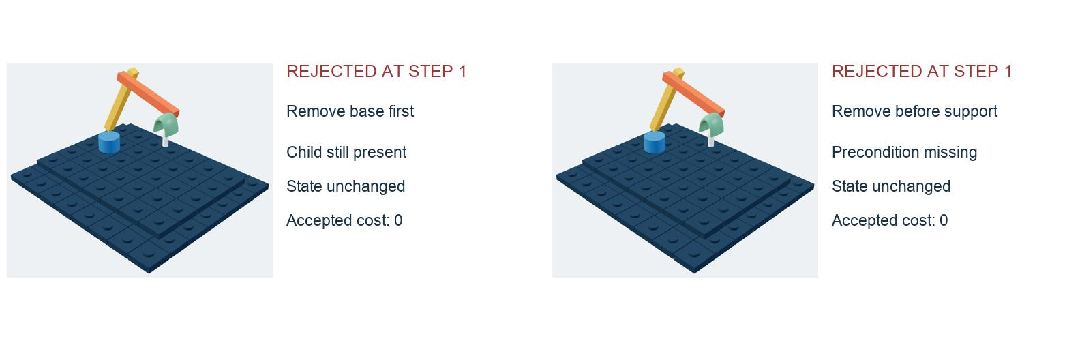
\includegraphics[width=.95\textwidth]{figures/publication-invalid.pdf}
\end{center}
\noindent\textbf{Failure examples.}
The program \texttt{remove:foundation} fails disassembly because
the mount is still present. The program \texttt{remove:cell-0-tool}
fails service repair because \texttt{done:open:cell-0-tool} is missing.
Both failures occur at step one, preserve the initial state, and
consume zero accepted cost. Identical appearance therefore does not
imply that a submitted step was accepted.

\begin{center}\small
\begin{tabularx}{\textwidth}{llX}
\toprule Output & Required fields & Acceptance condition\\\midrule
Single choice & \texttt{choiceId} & Match the designated option ID.\\
Choice set & \texttt{choiceIds} & Return exactly the full set, with valid unique IDs; order is ignored.\\
Action program & \texttt{actionIds} & Every transition legal, total cost within budget, terminal goals satisfied.\\
Schedule & \texttt{starts} & All jobs have integer starts, precedence and resources hold, deadline met.\\
Policy & \texttt{queryId}, \texttt{decisions} & Query within budget; action correct for every world's observation.\\
\bottomrule
\end{tabularx}
\end{center}

\subsection{English Worked Prompts}
\begin{enumerate}
\item \textbf{Atomic removal:} ``Which module can be removed without
leaving a direct child attached?'' Use the public alternatives and
return the option ID corresponding to the valid leaf set. In the
illustrated chain, the leaf is \texttt{cell-0-tool}.
\item \textbf{Procedural disassembly:} ``Submit action IDs that remove
every module while respecting the public prerequisites and budget.''
Return \texttt{remove:cell-0-tool}, \texttt{remove:cell-0-wrist},
\texttt{remove:cell-0-elbow}, \texttt{remove:cell-0-shoulder},
\texttt{remove:cell-0-mount}, \texttt{remove:foundation} in the
\texttt{actionIds} array.
\item \textbf{Service repair:} ``Execute the public service contract
and reach the repaired goal within seven actions.'' Return the seven
action IDs from the preceding table, each suffixed by
\texttt{:cell-0-tool}.
\item \textbf{Integrated resource repair:} ``Repair the tool and wrist
using the shared exclusive tool.'' This task has a distinct catalog:
isolate, support, unlock, replace, verify, relock, release for each
target. A valid reference program completes one target before
acquiring the tool for the other, requiring fourteen actions.
\end{enumerate}
These are explanatory translations of released task intents. Choice
letters must be read from the actual per-task alternatives, whose order
is deterministic but varies with task identity.

\subsection{Diagnostic Results and Denominators}
\begin{center}\small
\begin{tabularx}{\textwidth}{lrrX}
\toprule Check or experiment & Passed & Evaluated & Interpretation\\\midrule
Reference-answer replay & 6,912 & 6,912 & Construction and validator consistency.\\
Public-precondition action solver & 1,152 & 1,152 & Executability with public symbolic rules.\\
Constant A / empty choice set & 1,340 & 5,328 & Measured choice-only control, 25.15\%.\\
Constant / empty, all formats & 1,340 & 6,912 & Full-set control, 19.39\%.\\
GPT-4.1 mini, historical & 7 & 16 & Fixed base-48 pipeline pilot, not expanded-set accuracy.\\
Malformed-field diagnostic & 4 & 4 & Failed action outputs execute after post-hoc field renaming.\\
\bottomrule
\end{tabularx}
\end{center}
The historical pilot's nine strict failures consist of four schema
failures, four expected-loss errors, and one coordinate-transform
error. The diagnostic does not revise the official 7/16 score.
No population confidence interval or level ranking is inferred from
one response per level/layer cell.

\clearpage
\section{Answer Concentration and Program Length}
\begin{center}\small
\begin{tabular}{llrrr}
\toprule Family & Output format & Instances & Majority (\%) & Action steps\\\midrule
\tableinput{tables/publication-families.tex}
\bottomrule
\end{tabular}
\end{center}
Majority is the most frequent semantic answer among 144 instances of
a family. Single-choice option letters are removed before counting;
sets are canonicalized. Program rows count exact reference sequences,
including object-specific IDs, so their low concentration does not
imply diverse planning algorithms. Steps are min--max reference lengths,
not proven optimal lengths. The 100\% \texttt{no-op} majority and high
\texttt{degree}/\texttt{anchor} majorities limit those families'
discriminative value. These diagnostics are computed on the public
set and are not trained-baseline generalization results.

\clearpage
\section{Reproducing the Publication Artifacts}
The publication analysis reads the archived expanded models, controls,
answer distributions, and historical pilot. Its output
\texttt{publication-analysis.json} binds input hashes and supplies the
structural, control, and family tables. The replay capture manifest
binds the source model, renderer, interpreter, every frame's state,
and the corresponding image hash. The figure manifest binds raw images,
composition code, ASCII-only labels, and final plates.

\begin{verbatim}
node node_modules/tsx/dist/cli.mjs benchmark/paper/analyze-publication.ts
node node_modules/tsx/dist/cli.mjs benchmark/paper/capture-publication.ts
python3 benchmark/paper/compose-publication.py
cd benchmark/paper
../.runtime/tectonic --keep-logs main.tex
../.runtime/tectonic --keep-logs supplement.tex
python3 check_pdf.py
python3 check_pdf.py --paper supplement
node verify-artifacts.mjs
\end{verbatim}
Capture requires the original application running at port 5173
(or the \texttt{BRICKATLAS\_URL} override). The commands make no paid
inference calls and do not submit human review decisions. PDF checks
cover page geometry, overflow, unresolved references, CJK text, and
image inclusion; visual review remains a separate check of legibility.
The Chinese companion is distributed separately and is not embedded
in either English PDF.

\subsection{Interpretation of Physical Measurements}
\begin{center}\small
\begin{tabularx}{\textwidth}{lrrX}
\toprule Quantity & Maximum observed & Gate & Interpretation\\\midrule
Representative-point drift & 0.05305 & 0.35 & Translation during the nominal servo-held run.\\
Angular drift (rad) & 0.01825 & 0.15 & Rotation during the same nominal run.\\
Non-spring joint residual & 0.000815 & 0.02 & Declared joint consistency after settling.\\
Initial penetration & $\leq0.005$ & 0.005 & Oriented-cuboid inter-module gate.\\
\bottomrule
\end{tabularx}
\end{center}
Displayed maxima are rounded upward. All 144 configurations pass the
declared nominal protocol. This table is neither a material-calibration
result nor a guarantee of passive stability, continuous-motion validity,
or manufacturability. The complete object index follows.
